%%=============================================================================
%% Methodologie
%%=============================================================================

\chapter{\IfLanguageName{dutch}{Proof-of-concept}{Proof-of-concept}}%
\label{ch:proof-of-concept}

\subsubsection{Inleiding}
Dit hoofdstuk licht het ontwerp en de opbouw van de proof-of-concept toe.

\section{Toelichting}
Bij de voorbereiding van de proof-of-concept zijn bepaalde beslissingen genomen met betrekking tot het ontwerp en de architectuur van het project. Deze toelichting heeft als doel uit te leggen en te verduidelijken waarom die beslissingen zijn genomen.

\begin{itemize}
    \item Gebruik van een Arduino
    
    Elk van de printers in een kopieercentrum is aangesloten op de Arduino UNO. De Arduino UNO is gekozen omdat deze volledig programmeerbaar is. Op dit moment pikt deze Arduino gewoon de analoge klik van een printer op en stuurt een digitaal signaal met een kleine payload naar de Raspberry Pi. In deze payload zit alleen het pinnummer waarop de klik is ontvangen. In de toekomst kan deze payload worden uitgebreid met meer informatie. Dit is mogelijk dankzij de programmeerbaarheid van de microcontroller.
    
    \item Gebruik van een Raspberry Pi
    
    Het gebruik van een Raspberry Pi als server heeft een aantal voordelen ten opzichte van een standaardcomputer.
    Eerst en vooral is de Raspberry Pi voordeliger in gebruik aangezien deze een ARM-processor gebruikt. Dit komt omdat de Raspberry Pi een ARM-processor gebruikt. Deze is veel goedkoper dan een normale processor.
    
    Het tweede grote voordeel van de Raspberry Pi is zijn energieverbruik. In feite is zijn stroomverbruik veel lager dan dat van de gemiddelde desktopcomputer. Dit is vooral te danken aan de eerdergenoemde ARM-processor.
    
    Tot slot is ook de flexibiliteit van een Raspberry een groot voordeel. Dankzij de flexibiliteit van de Raspberry Pi kan hij in het proof of concept voor verschillende dingen worden gebruikt zoals onder meer om te luisteren naar de digitale signalen die de Arduino UNO uitzendt en om een aantal microservice containers in Docker te draaien.
    
    \item Toepassen van de microservices architectuur
    
    De toepassing van de microservices architectuur brengt een paar voordelen met zich mee, namelijk: schaalbaarheid en veerkrachtigheid.
    
    Eerst en vooral zijn microservices heel erg schaalbaar.    
    Goossens NV heeft plannen om de copycentra in de toekomst uit te breiden. Dit kan ervoor zorgen dat de operations API overbelast kan raken op piekmomenten. Dankzij het feit dat deze API opgezet is als microservice, is het mogelijk om deze service horizontaal te schalen. Concreet wil dit zeggen dat er meerdere instanties van deze service naast elkaar zullen draaien en worden de aanvragen over de verschillende instanties gespreid. Wanneer het piekmoment voorbij is, worden de overtollige services terug verwijderd.
    
    Daarnaast zijn microservices ook heel erg veerkrachtig.
    Tijdens de proof-of-concept werden twee verschillende API's gebouwd. Terwijl een eerste wordt gebruikt om de printers en diens staffels te managen, dient een tweede om de dagelijkse operaties te ondersteunen. In de toekomst kunnen er extra API's worden ontwikkeld en uitgerold in de winkels. Dankzij de veerkrachtigheid van de microservices kan één van de microservices crashen of offline gehaald worden zonder de andere services in het gedrang te brengen.
    
    \item Gebruik van python bij het listener script
    Python heeft ingebouwde bibliotheken voor het lezen van en schrijven naar de seriële bus in Python. Omdat de Arduino serieel verbonden is met de Raspberry Pi waarop de listener zal draaien, is het luisteren naar seriële bussen belangrijk. Het doel van deze luisteraar is het lezen van seriële busberichten en het decoderen van de payload in het bericht.
    Bibliotheken voor het versturen van verzoeken naar een REST API zijn ook opgenomen in de programmeertaal Python. Na decodering en validering van de ontvangen payload moet het script een PATCH-verzoek sturen naar de Operation API met het nummer dat uit de payload is verkregen als parameter.
\end{itemize}

\section{Domeinarchitectuur}
\begin{figure}[H]
    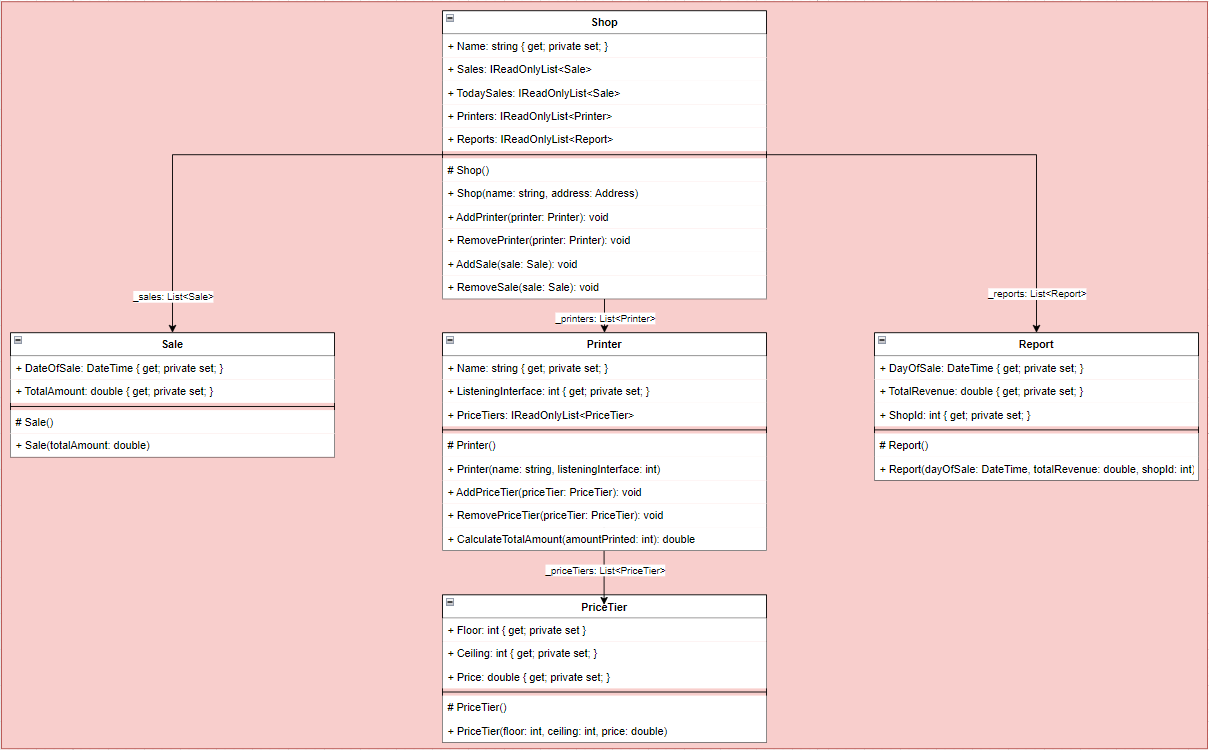
\includegraphics[scale=0.50]{domain_diagram}
    \centering
    \caption{Schematische voorstelling van het domein}
    \label{fig:domainArchitecture}
\end{figure}

Het domein van deze proof-of-concept bestaat uit vijf klassen: Shop, Sale, Printer, Report en PriceTier.

\begin{itemize}
    \item Shop
    
    De Shop klasse heeft volgende eigenschappen:
    
    \begin{itemize}
        \item Naam (\textit{Name}-property): de naam van de winkel.
        \item Verkopen (\textit{Sales}-property): een lijst van verkopen die plaatsgevonden hebben in de winkel.
        \item Verkopen van vandaag (\textit{TodaySales}-property): een sublijst van verkopen die vandaag hebben plaatsgevonden in de winkel.
        \item Printers (\textit{Printers}-property): een lijst van aanwezige printers in de winkel.
        \item Reports (\textit{Reports}-property): een lijst van rapporten gekoppeld aan de winkel.
    \end{itemize}

    Als ook volgende methoden:
    \begin{itemize}
        \item Toevoegen van een printer (\textit{AddPrinter}-method): een methode voor het toevoegen van een printer aan de winkel.
        \item Verwijderen van een printer (\textit{RemovePrinter}-method): een methode voor het verwijderen van een printer uit de winkel.
        \item Toevoegen van een verkoop (\textit{AddSale}-method): een methode voor het toevoegen van een verkoop aan de winkel.
        \item Verwijderen van een printer (\textit{RemovePrinter}-method): een methode voor het verwijderen van een verkoop uit de winkel.
    \end{itemize}

    \item Sale
    
    De Sale klasse bevat volgende eigenschappen:
    
    \begin{itemize}
        \item Datum van verkoop (\textit{DateOfSale}-method): de datum waarop de verkoop heeft plaatsgevonden.
        \item Totaal betaald bedrag (\textit{TotalAmount}-method): het totaal betaald bedrag.
    \end{itemize}
    
    \item Printer
    
    De Printer klasse bestaat uit deze eigenschappen:
    
    \begin{itemize}
        \item Naam (\textit{Name}-property): de naam van de printer.
        \item Geregistreerd Arduino pinnummer (\textit{ListeningInterface}-property): het pinnummer waarop de printer geconnecteerd is met de Arduino UNO.
        \item Prijsstaffels (\textit{PriceTiers}-property): een lijst van prijsstaffels voor de printer.
    \end{itemize}

    En volgende methoden:
    \begin{itemize}
        \item Toevoegen van een prijsstaffel (\textit{AddPriceTier}-method): een methode voor het toevoegen van een prijsstaffel aan een printer.
        \item Verwijderen van een prijsstaffel (\textit{RemovePriceTier}-method): een methode voor het verwijderen van een prijsstaffel uit een printer.
        \item Bereken totaal te betalen bedrag (\textit{CalculateTotalAmount}-method): een methode voor het berekenen van de prijs op basis van de huidige actieve prijsstaffel.
    \end{itemize}
    
    \item Report
    
    De Report klasse heeft deze eigenschappen:
    
    \begin{itemize}
        \item Datum van verkoopdag (\textit{DayOfSale}-property): de datum van het dagrapport.
        \item Totale opbrengst (\textit{TotalRevenue}-property): de totale omzet die gedraaid werd die dag.
        \item Winkel identificatie (\textit{ShopId}-property): het unieke nummer waarmee de winkel, waarover het dagrapport gaat, identificeerbaar is.
    \end{itemize}

    \item PriceTier
    
    De PriceTier klasse omvat volgende eigenschappen:
    
    \begin{itemize}
        \item Ondergrens (\textit{Floor}-property): de inclusieve ondergrens van de staffel.
        \item Bovengrens (\textit{Ceiling}-property): de inclusieve bovengrens van de staffel.
        \item Prijs (\textit{Price}-property): de prijs gekoppeld aan deze staffel.
    \end{itemize}
    
\end{itemize}

\section{Systeemarchictectuur}
%TODO: check afbeelding
\begin{figure}[H]
    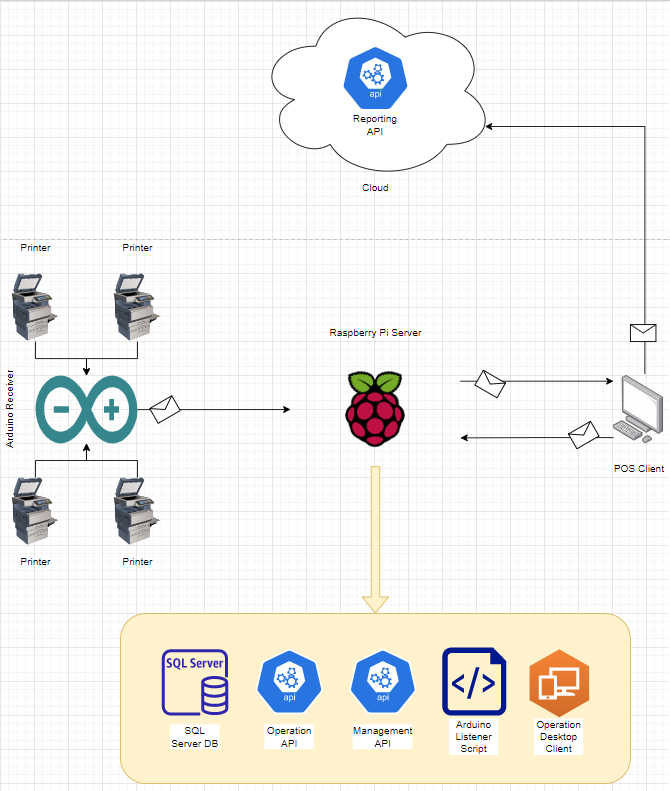
\includegraphics[scale=0.75]{system_architecture}
    \centering
    \caption{Schematische voorstelling van de systeemarchitectuur}
    \label{fig:systemArchitecture}
\end{figure}

Deze proof-of-concept is gebasseerd op de huidige systeemarchitectuur binnen de copycentra van Goossens NV. Momenteel zijn alle printers binnen één copycenter allemaal geschakeld aan één schakelbord. Dit bord staat dan op zijn beurt in verbindingen met het kassasysteem. Het doel van dit bord is om de analoge klik die een printer uitstuurt na het printen van een bladzijde op te vangen en door te geven aan het kassasysteem.

In de nieuwe systeemarchitectuur (afgebeeld in Figuur 4.1) staan alle printers geschakeld aan een Arduino Uno. Het doel van deze Arduino is het opvangen van het analoge signaal en een digitaal signaal uit te sturen via een seriële verbinding. Deze seriële verbinding mondt uit in een Raspberry Pi, waar verschillende microservices draaien:

\begin{itemize}
    \item Microsoft SQL Server
    
    De Microsoft SQL Server service fungeert als centrale databank waar alle microservices hun data kunnen wegschrijven en ophalen.
    
    \item Management API
    %TODO: check methoden
    
    De Management API heeft als doel het managen van de printers en hun staffels. Onder het managen van printers wordt het aanmaken en verwijderen van printers binnen één winkel begrepen. Het managen van de printerstaffels houdt het aanmaken, verwijderen en bijwerken van printerstaffels voor één printer in.
    
    \item Arduino Listener script
    
    Dit script is geschreven in python en heeft als doel de seriële bus van de Raspberry Pi uit te lezen. Op deze seriële bus staan de boodschappen uitgestuurd door de Arduino Uno. Ieder bericht bevat een kleine payload die aangeeft welke op welke interface van de Arduino de analoge klik is binnengekomen. Na het decoderen van de payload, stuurt het script een PATCH-aanvraag naar de Operation API.
    
    \item Operations API
    
    Deze API is bedoeld om de dagdagelijkse operaties te ondersteunen. Deze haalt alle data op die nodig is voor de desktop kassa-applicatie, berekent het totaal te betalen bedrag, schrijft alle verkopen weg naar de databank, ontvangt de PATCH-aanvragen van het Arduino Listener script en stuurt update commando's uit naar de desktopapplicatie.
    
    \item Operation Desktop Client
    
    Dit is bedoeld als GUI (Graphical User Interface) voor de verko(o)p(st)ers van de copycentra. Hier wordt de huidige tellerstand van de printers bijgehouden. Indien een klant wil afrekenen, kan de winkelverantwoordelijke dit snel en eenvoudig en de betaling registreren. Op het einde van de dag wordt deze GUI afgesloten en wordt het dagrapport gegenereerd.
    
    \item Reporting API
    
    Deze API wordt gebruikt om de dagrapporten te genereren wanneer een kassasysteem afgesloten worden. Na het genereren van het dagrapport wordt er door deze API een push-notificatie uitgestuurd naar de Reporting applicatie om de gebruiker te laten weten dat er een nieuw dagrapport beschikbaar is.
    
    \item Reporting Client
    
    Deze applicatie laat toe om de data aangeleverd door de dagrapporten te visualiseren in verschillende grafieken te kunnen bekijken en zo een overzicht te verschaffen hoe de winkels het op vlak van omzet doen.
\end{itemize}